% Full title as you would like it to appear on the page
\chapter{Tabula Sapiens: A molecular atlas of human cells}
% Short title that appears in the header of pages within the chapter
\chaptermark{Tabula Sapiens}

\section{Abstract}
Single-cell transcriptome sequencing will help biologists understand the molecular characteristics and physiological functions of human organs. In this study, we constructed the Tabula Sapiens, a comprehensive human reference atlas containing nearly 500,000 cells from 24 distinct tissues and organs. My analysis enabled the molecular characterization of over 250,000 immune cells, their distribution across tissues, and tissue-specific gene expression variations. By examining multiple tissues from a single donor, I investigated the clonal distribution of T cells, tissue-specific mutation rates in B cells, and tissue-specific gene expression programs of multiple cell types. The Tabula Sapiens provides a valuable resource for studying gene expression programs and lineage histories of shared cell types across tissues, opening up new avenues for understanding human physiology and disease. The clone tracing I performed in T cells in this work is an important proof-of-concept for the following chapters, where I use lineage tracing of B cells to gain insight into the dynamics of the human immune system. 

\section{Introduction}

The Tabula Sapiens project represents a significant milestone in the study of human biology\ref{fig:paper1_summary}. By leveraging cutting-edge technologies such as single-cell capture via microfluidics, high throughput DNA/RNA sequencing, and immune repertoire sequencing, this project provides researchers with valuable insights into cellular taxonomy, tissue structure, cell fate and lineage, and cellular communication. Ultimately, the Tabula Sapiens project can revolutionize our understanding of human biology, inform the development of novel therapeutic strategies, and facilitate early detection and diagnosis of various diseases. Importantly, this effort is mainly a reading project. We generated a parts-list for human biology at unprecedented scale and depth. However, a revolution in biology critically depends upon our ability to write biological information and reprogram cells at a similar scale.  

\begin{figure}[hbt!]
\centering
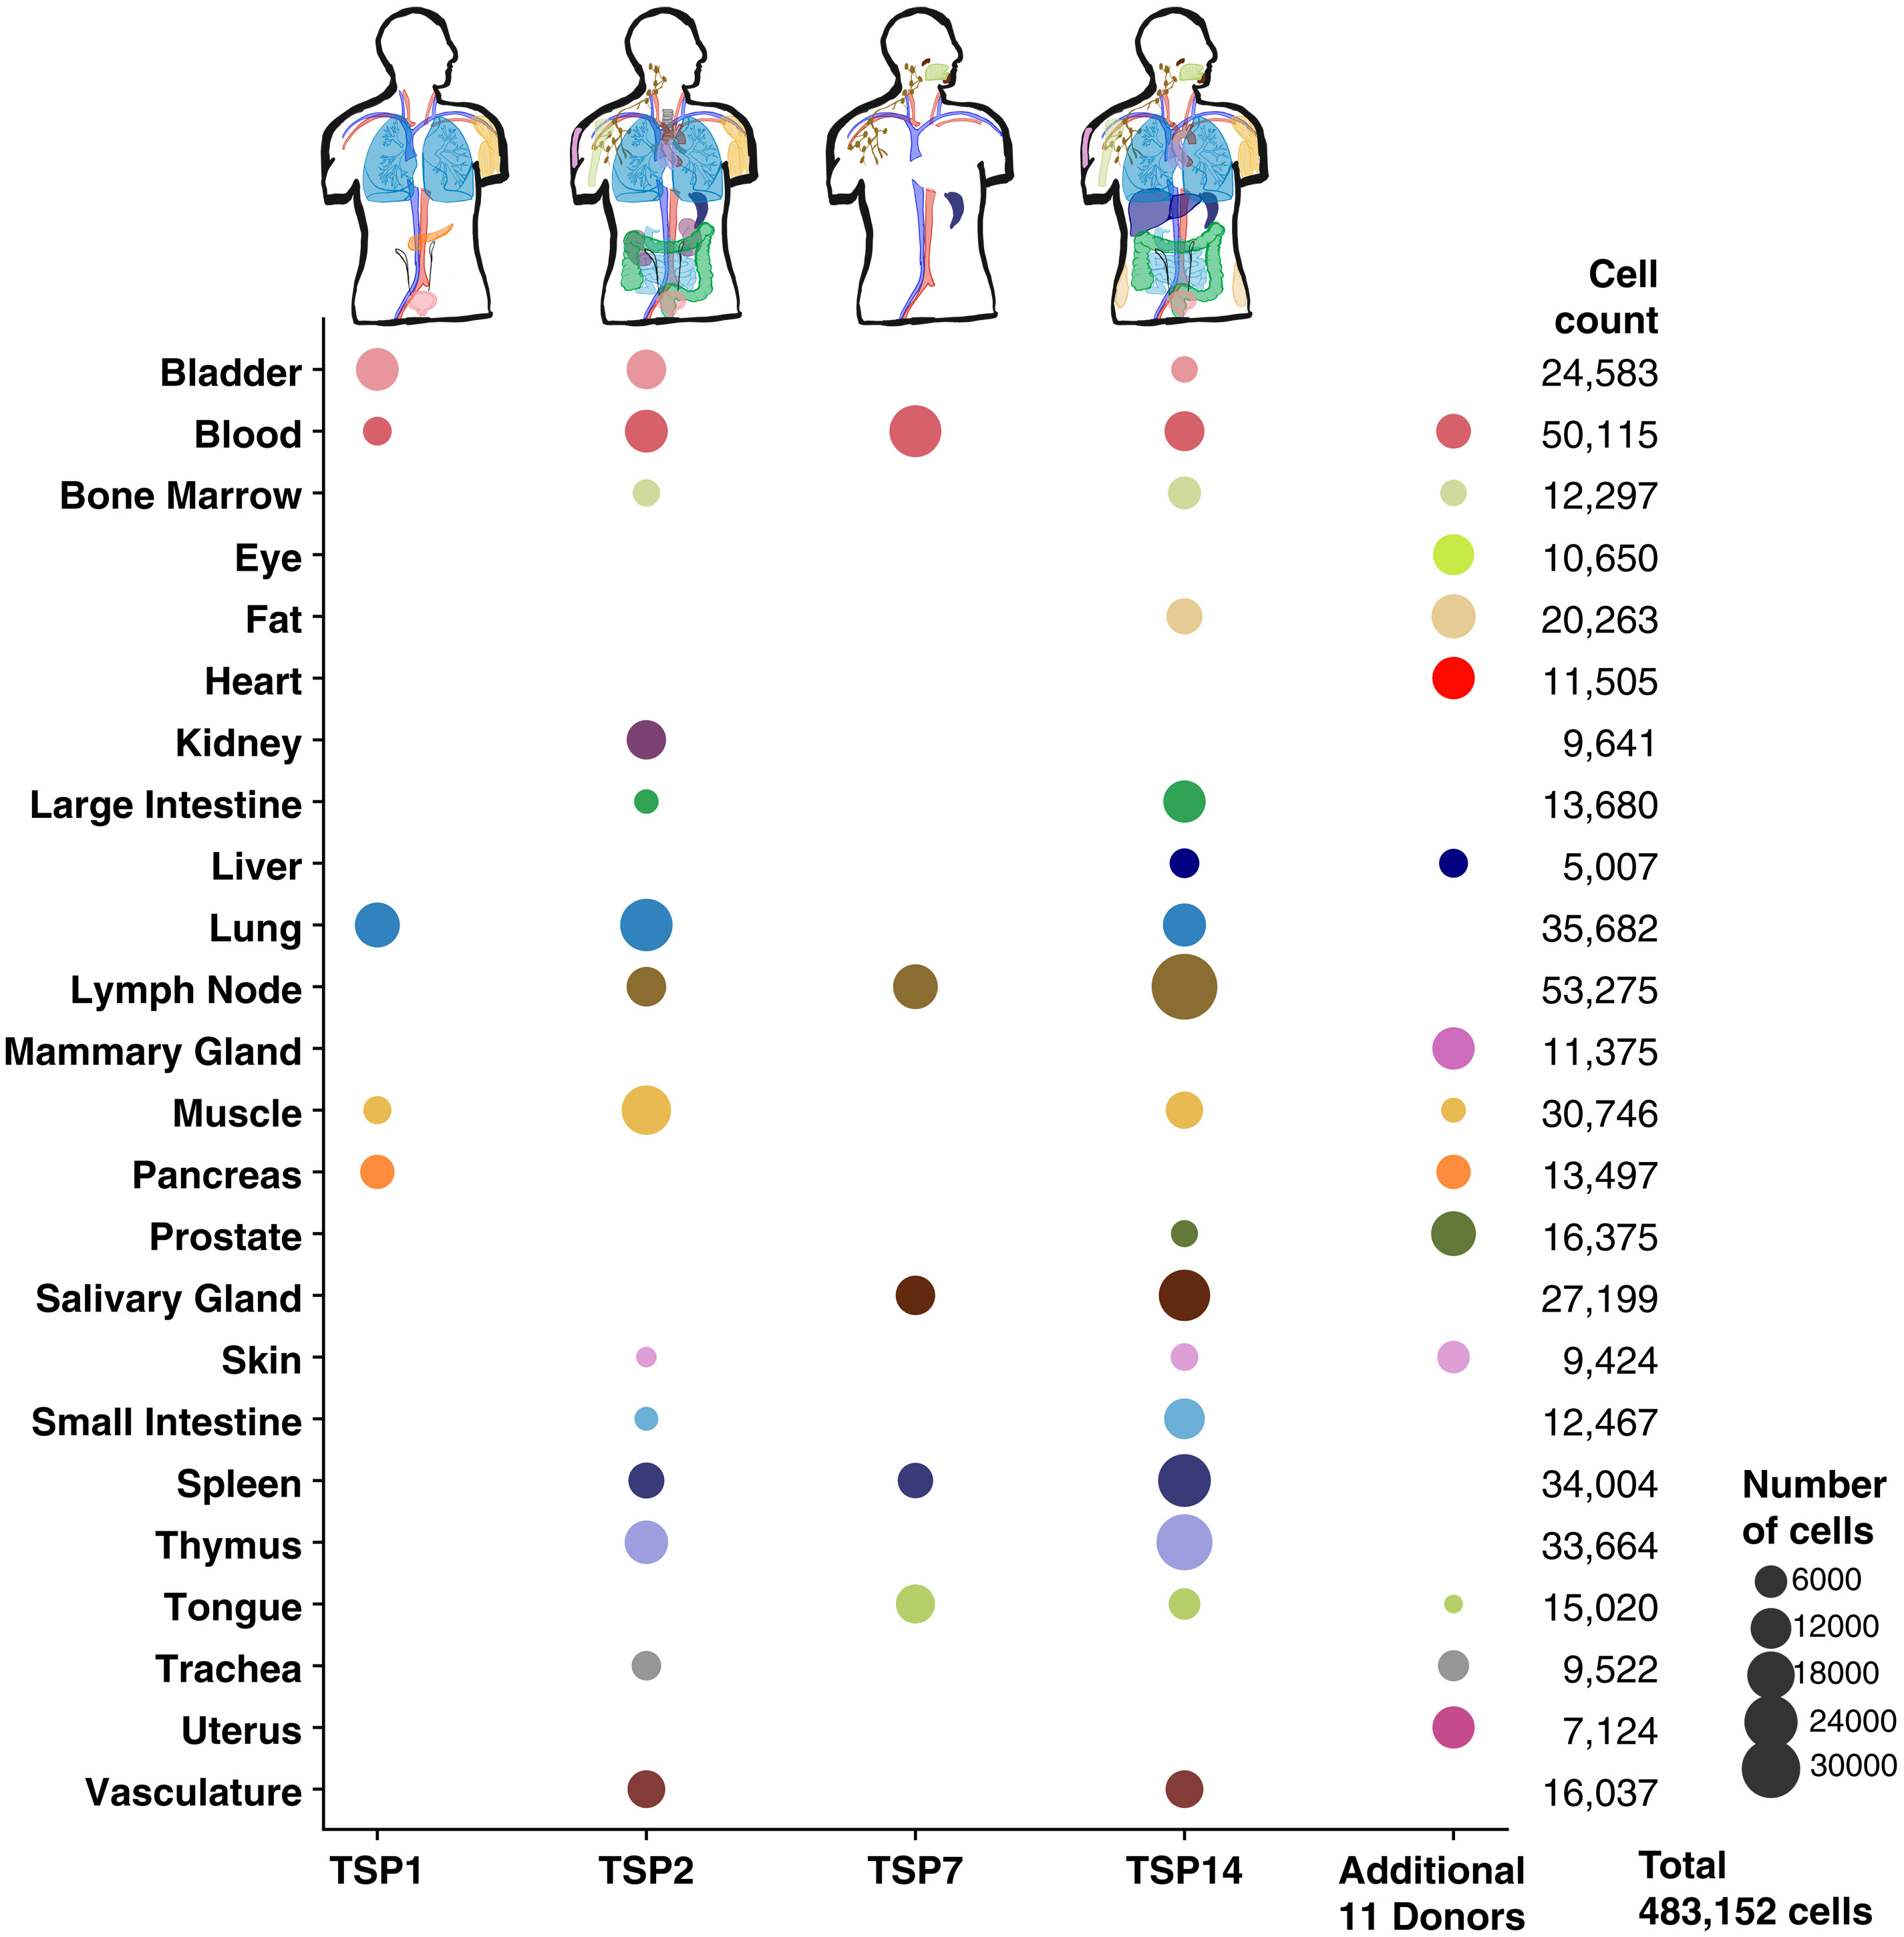
\includegraphics[width=14cm, keepaspectratio]{figs/paper1/fig0_Tabula_Summary.jpg}
\caption[ Overview of Tabula Sapiens.]{The Tabula Sapiens was constructed with data from 15 human donors; for detailed information on which tissues were examined for each donor, please refer to table S2. Demographic and clinical information about each donor is listed in the supplementary materials and methods and in table S1. Donors 1, 2, 7, and 14 contributed the largest number of tissues each, and the number of cells from each tissue is indicated by the size of each circle. Tissue contributions from additional donors who contributed single or small numbers of tissues are shown in the additional 11 donors column, and the total number of cells for each organ are shown in the final column on the right.}
\label{fig:paper1_summary}
\end{figure}

\subsection{Motivation for the Tabula Sapiens}

Our knowledge of the cells that make up the human body, as well as their variations across individuals, developmental stages, and health or disease states, remains limited. The Human Cell Atlas (HCA) initiative is loosely-affiliated global collaboration involving scientists from numerous universities and institutes. Tabula Sapiens is a part of this broader effort, which aims to address this knowledge gap by creating comprehensive reference maps of all human cells\cite{regev2017human} These maps will serve as a foundation for research, diagnosis, monitoring, and treatment, providing crucial insights into cellular taxonomy, histology, developmental biology, physiology, and even comparative evolution.

Technological advancements have allowed the construction of a systematic molecular atlas at an unprecedented resolution. Single-cell RNA sequencing, for example, now the measurement of  mRNA profiles for millions of individual cells\cite{svensson2017power}. Other techniques, such as those assessing protein molecules\cite{stoeckius2017simultaneous} and chromatin accessibility (cite), further contribute to the wealth of information obtained from each cell. These tools have already shown tremendous potential in early studies, leading to the discovery of new cell types in various organs and tissues and providing insights into the immune system and tumor ecosystems\cite{regev2017human}.

\subsection{Tabula Sapiens and the Development of Key Technologies}

The Tabula Sapiens project builds upon the foundation laid by the HCA initiative, taking advantage of recent technological advancements in single-cell capture, sequencing, and immune repertoire sequencing. Microfluidics-based single-cell capture techniques have revolutionized the isolation and analysis of individual cells, allowing for the high-throughput processing and in-depth investigation of cellular heterogeneity\cite{macosko2015highly}. DNA/RNA sequencing technologies have similarly evolved, enabling the rapid and cost-effective characterization of an organism's entire genome or transcriptome\cite{goodwin2016coming}. Immune repertoire sequencing has also seen significant progress, facilitating the in-depth exploration of adaptive immune responses by analyzing the diversity of B and T cell receptors\cite{georgiou_promise_2014}.

Together, these technologies have empowered researchers to embark on the Tabula Sapiens project, an endeavor that will greatly enhance our understanding of human biology and provide a foundation for future research, diagnosis, and treatment. The integration of these technologies will help address key challenges in diverse biological fields, as well as facilitate the development of better drugs and more accurate predictions of unintended toxicity. Ultimately, the Tabula Sapiens project will contribute to a more comprehensive understanding of human cells and their functions, driving innovation in regenerative medicine and diagnostic tests.

\subsection{My contributions to the project}
In this study, I made a significant contribution to the Tabula Sapiens project, a comprehensive effort to generate a human cell atlas covering all major tissues and cell types. My involvement in the project spanned from collecting tissues, to analyzing data,  and writing the manuscript. included three primary aspects: collecting tissues and creating single-cell suspensions including developing a protocol to isolate bone marrow cells from human vertebral bodies, generating and advising in the preparation of 10X Genomics libraries, and performing tissue-specific gene expression analysis and clonal analysis of T cells, as well as estimating important parameters of B cell population genetics across tissues.

First, I successfully developed a novel protocol to isolate bone marrow cells from human vertebral bodies, a challenging tissue source due to the intricate structure and limited accessibility of the vertebral bone marrow. This protocol enabled me to obtain a high-quality, representative cell population from this complex tissue, thereby enriching the Tabula Sapiens project with essential data on bone marrow cell types and their interactions. Additionally, I processed lymph nodes, spleens, and blood for various Tabula Sapiens donors.

Second, I played a crucial role in generating and troubleshooting 10X Genomics and Smart-seq2 libraries for the project. My expertise in scRNA-seq library preparation allowed me to generate the 10X 5prime data efficientlys and well as serve in a key advisory role for the rest of library preparation optimize conditions and workflow, ensuring the generation of high-quality, reproducible data.

Finally, I performed tissue-specific gene expression analysis and clonal analysis of T cells, as well as estimated important parameters of B cell population genetics across tissues. My tissue-specific analysis helped uncover unique gene expression patterns and functional states of T and B cells in different human tissues. I investigated the clonal relationships among T cells and provided a view into their tissue-specific expansion and functional roles. Additionally, I estimated key parameters of B cell population genetics, such as somatic hypermutation rates and class-switch recombination frequencies, across various tissues, providing a view of B cell dynamics in human health and disease. 


\section{Results}

\subsection{Tissue-Specific Gene Expression Signatures of Immune Cells}

We performed a differential gene expression analysis on the immune cell types across all of the tissues, revealing tissue-specific gene expression signatures of immune cells. Although we identified signatures of interest for most cell types in our dataset, here we focus here on the 36,475 macrophages distributed amongst 20 tissues. Using PCA on the top X differentially expressed genes in macrophage across all tissues, we show a number of highly distinct macrophage subtypes \ref{fig:paper1_gex}. PCA distinguished lung and lymph node macrophages from all other macrophages, driven largely by the high expression of CHIT1 and anti-microbial genes. Macrophage in the spleen were unique amongst tissues, expressing SPIC and CD5L. This suggests that most macrophages in the spleen are red-pulp macrophages. Additionally, we identified a gradient of EREG expression that distinguished tissues such as skin, uterus, and mammary tissues from circulating macrophages in the blood \ref{fig:paper1_gex}. EREG, secreted by macrophages, is thought to participate in cancer progression and facilitate the tumor micro-environment but also has important roles in homeostatic maintenance of tissues. We summarized our analysis by plotting a clustermap of gene expression signatures of the macrophages and their tissue-defining genes \ref{fig:paper1_gex}, and by providing the gene loadings of the first 4 principal components in our analysis \ref{fig:paper1_gex}.  
\begin{figure}[hbt!]
\centering
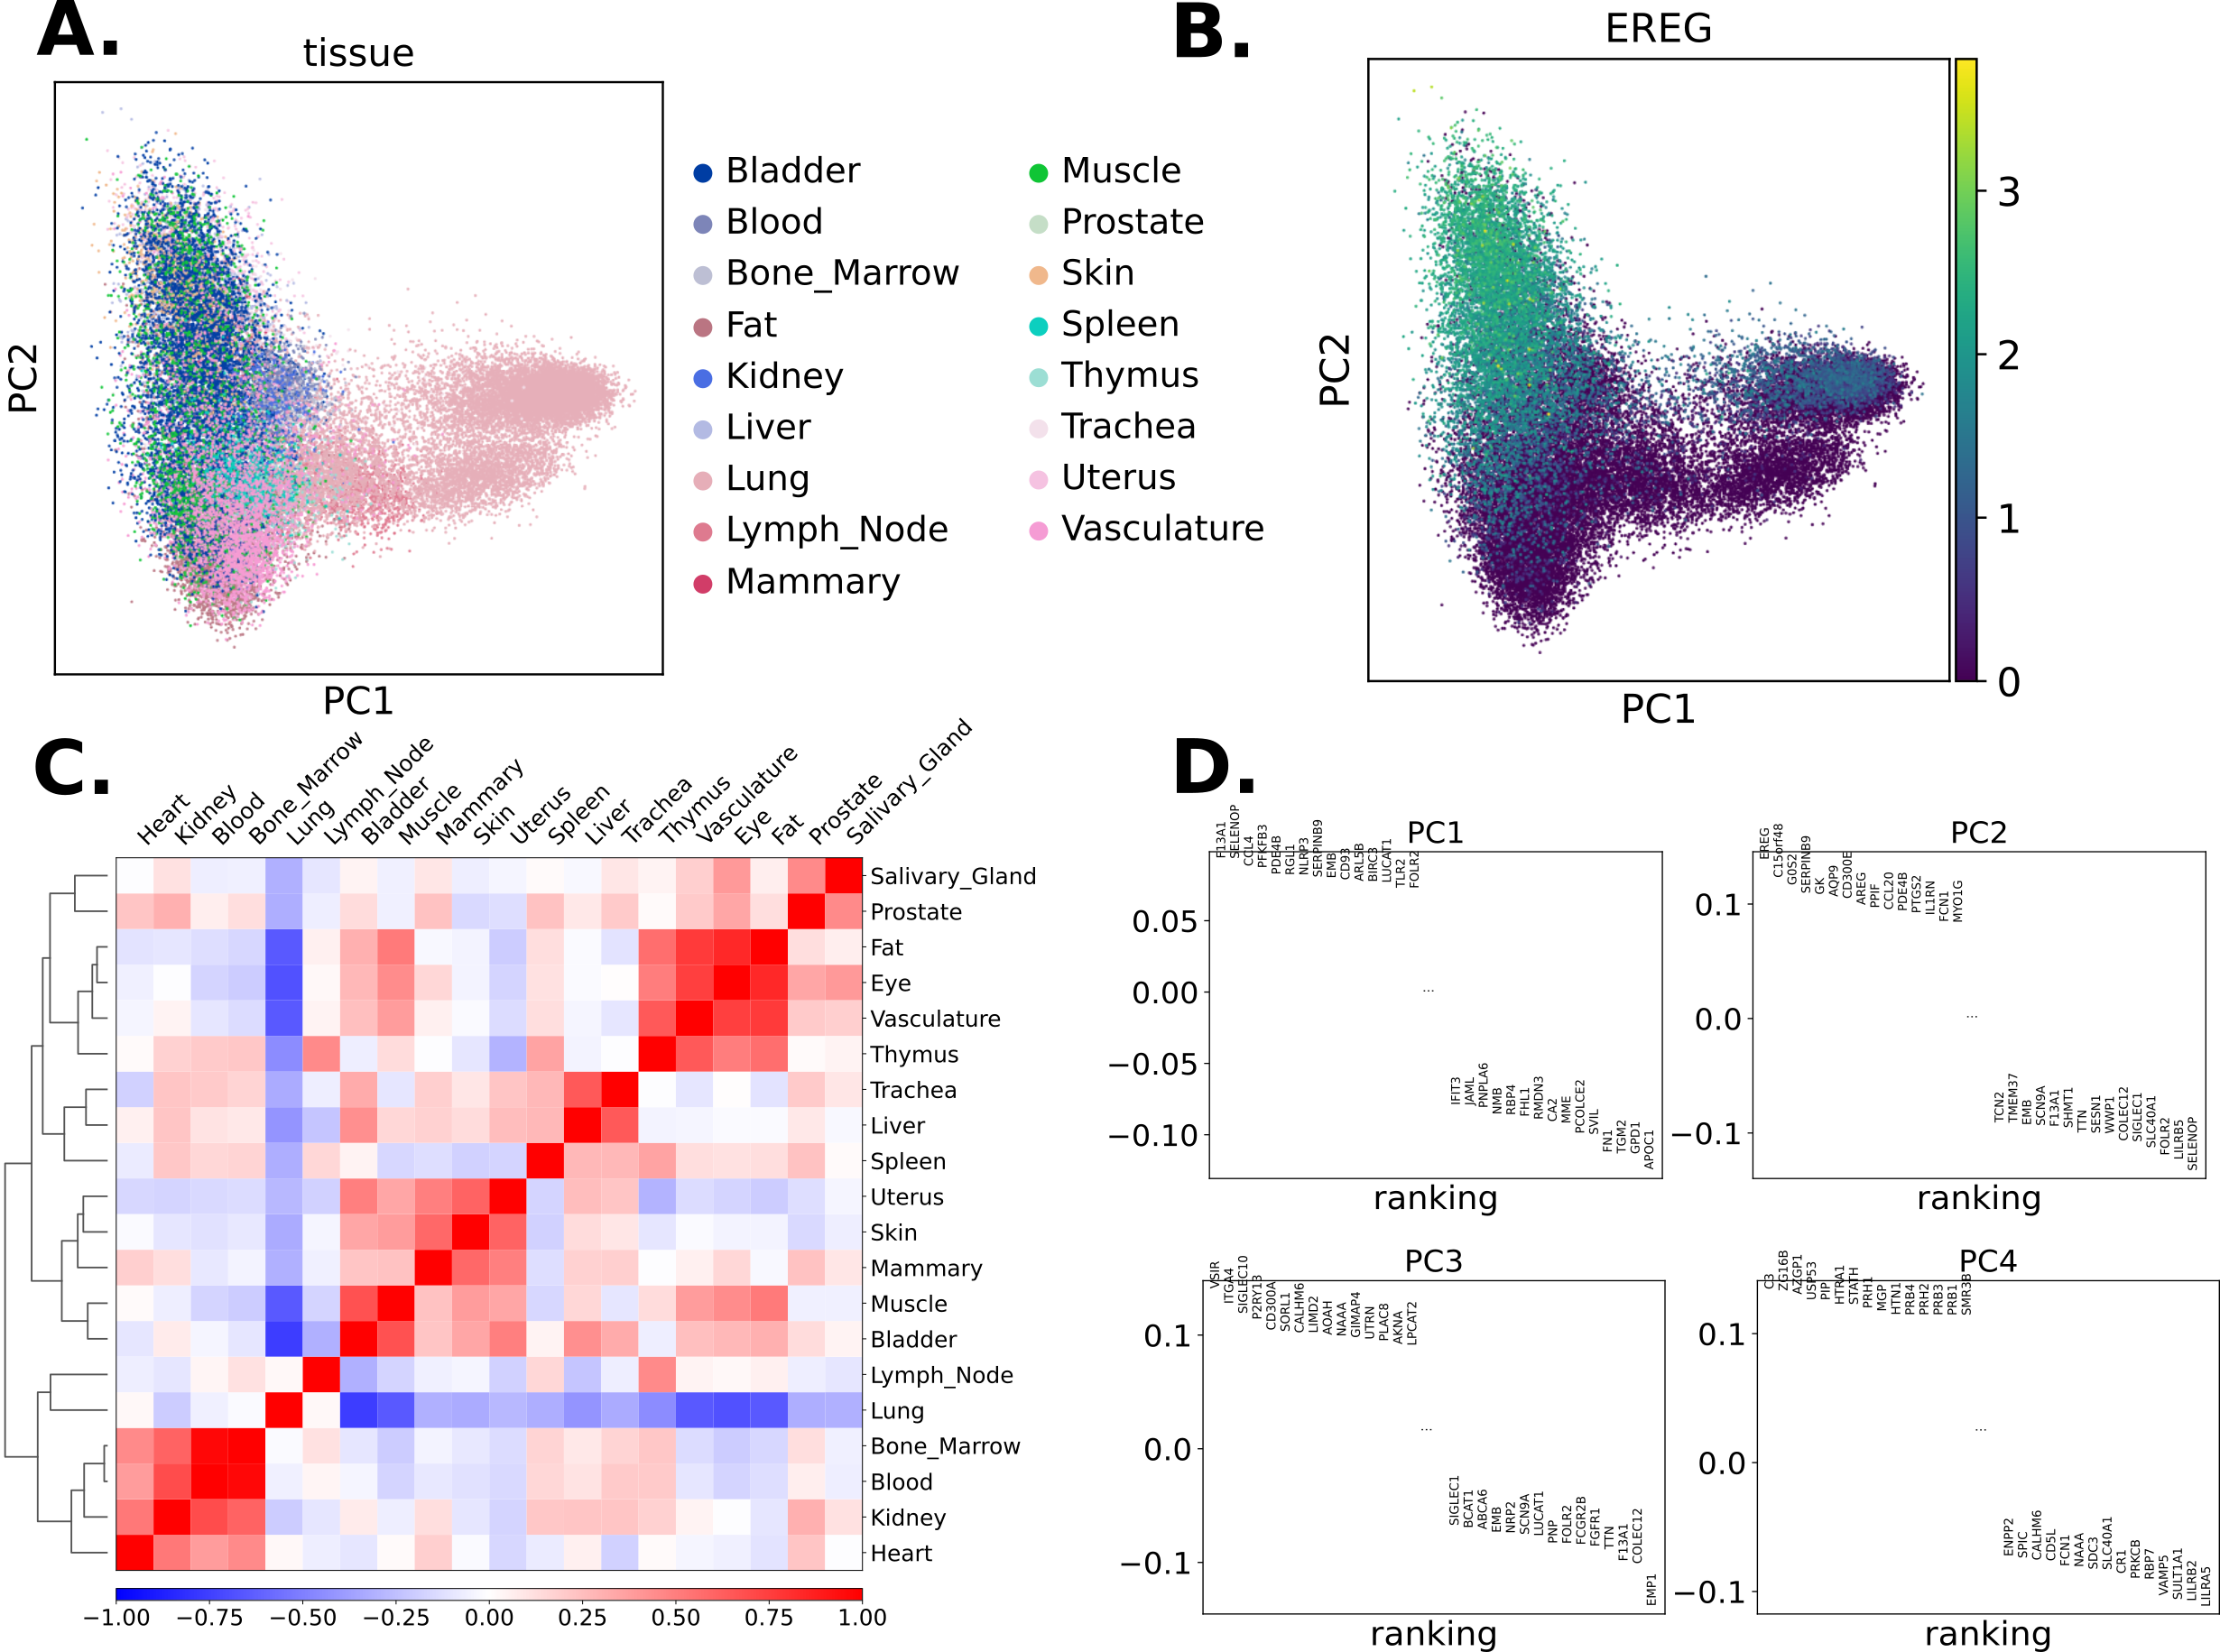
\includegraphics[width=14cm, keepaspectratio]{figs/paper1/fig1_gex_analysis.png}
\caption[Gene Expreesion Analysis of Tissue Resident Macrophage]{(A) PCA projection of the top 300 differentially expressed genes amongst macrophage amongst tissues. (B) Epiregulin expression defines macrophage residence in stromal tissues. (C) Correlation matrix of tissue resident macrophage gene expression. (D) Gene loadings of the first 4 principal components of gene expression variation amongst macrophage}
\label{fig:paper1_gex}
\end{figure}

\subsection{Immune Cell Trafficking Across Tissues}
Our analysis aimed to elucidate the molecular details of immune cell trafficking within individual humans by comparing different immune cell subsets across various tissues. These cells are known to originate in specific niches, circulate throughout the body, and home to other niches where they can remain for durations ranging from minutes\cite{jerison_heterogeneous_2020} to years\cite{hammarlund_plasma_2017}. The adaptive immune system is responsible for mounting a specific response to pathogens, with B cells producing antibodies and T cells orchestrating the immune response and directly attacking infected cells (3). Both B and T cells express unique receptors on their cell surface (BCRs and TCRS), which are created in a stochastic process which results in the creation of novel genes and gene combinations. Thus, lymphocytes are relatively uniquely marked at the time of their origin, such that observation of the same gene in two different cells is indicative of a clonal relationship between them (4). Of course, to identify these clones by their immune receptor, one needs to sequence the TCR or BCR. The techniques for sequencing TCRs and BCRs are called Airr-seq, or Adaptive Immune Receptor Repertoire sequencing. It is a high-throughput sequencing method that enables the in-depth analysis of the T cell receptor (TCR) and B cell receptor (BCR) repertoires of the adaptive immune system (1, 2). 

The BCR and TCR receptors are composed of two distinct chains (light and heavy for BCRs, and alpha and beta or gamma and delta for TCRs), which are paired to form the complete receptor (5) \ref{fig:paper1_airr}. 

\begin{figure}[hbt!]
\centering
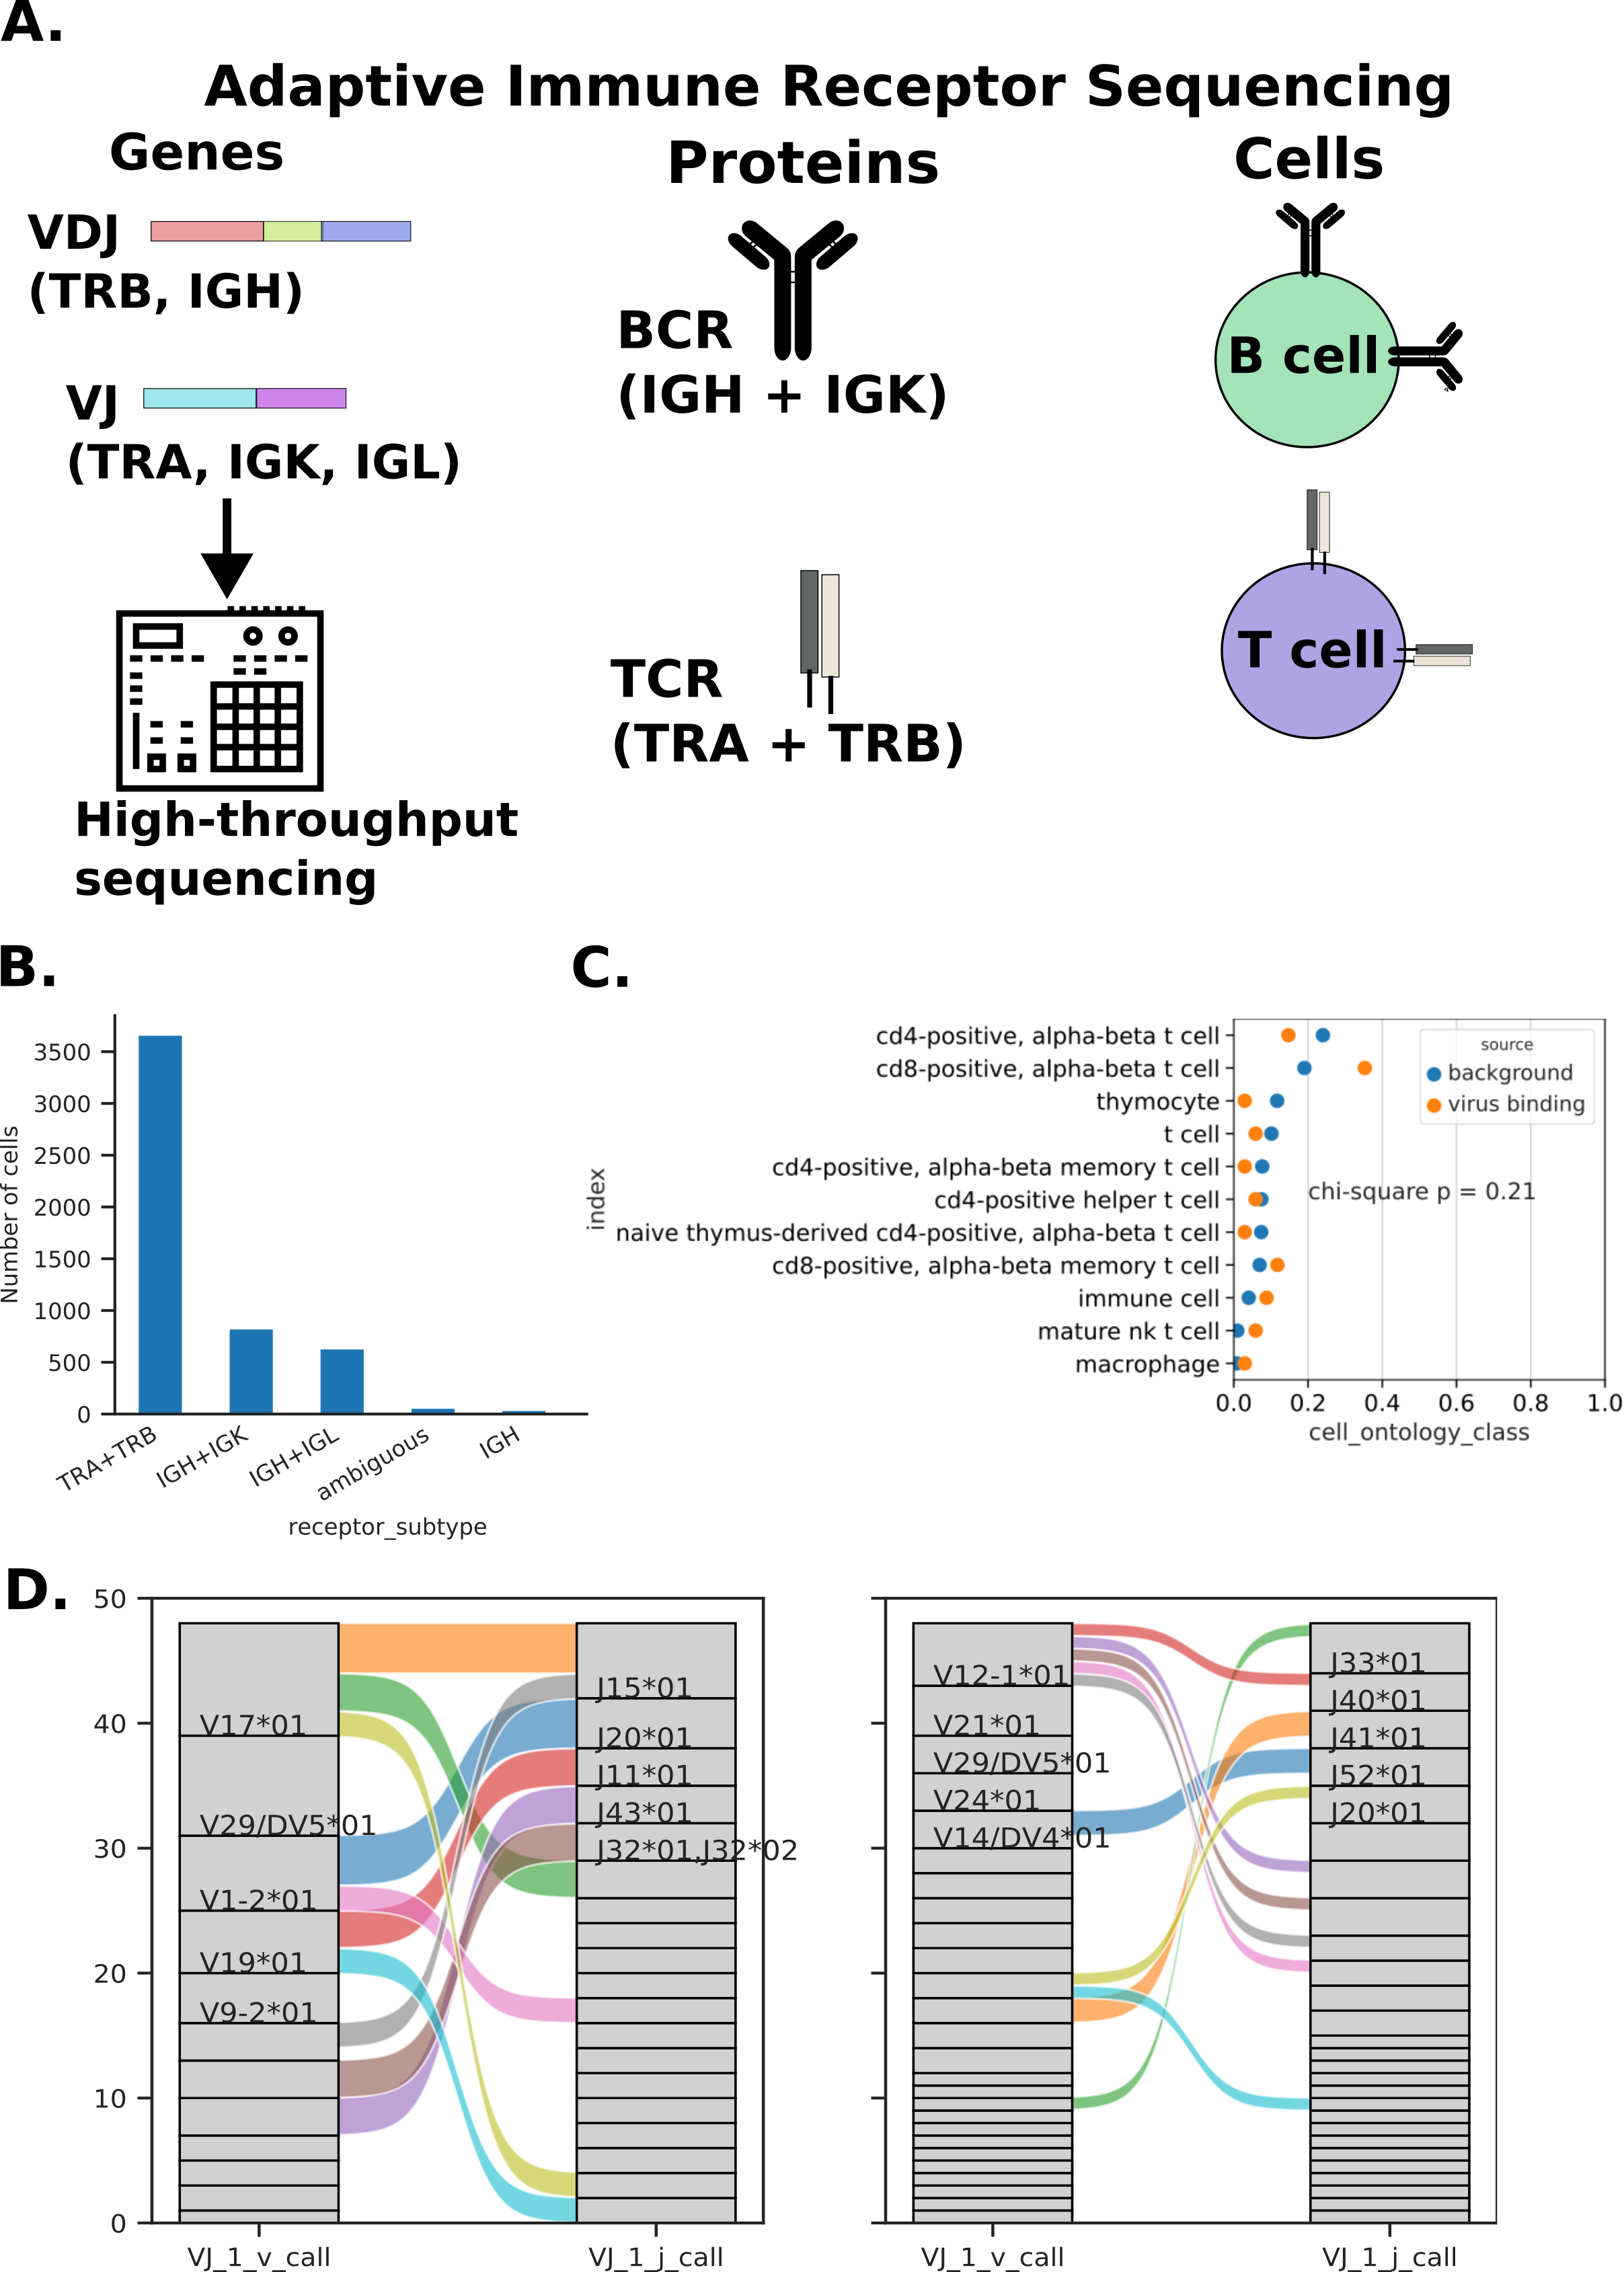
\includegraphics[width=11cm, keepaspectratio]{figs/paper1/fig2_tabula_airr.png}
\caption[AIRR-seq for analyzing the T cell Repertoire in Tabula Sapiens]{A. Schematic of Adaptive Immune Receptor Sequencing. B.Countplot of TCRs and BCRs which computationally assembled from Smart-Seq2 and 10X 5prime data using Bracer/Tracer and Cellranger respectively. These are assemblies for which a gene expression profile from the same cell was also found.MAIT cells and other invariant T cells use a stereotypical repertoire of V and J genes. Multi-donor T cell clones (left) tended to use a rescricted set of known MAIT genes as compared to the (downsampled) full T cell repertoire (left)}
\label{fig:paper1_airr}
\end{figure}

The pairing of the chains is essential for receptor functionality and antigen recognition. Single-cell sequencing approaches have proven to be beneficial for analyzing immune repertoires, as they allow for the simultaneous sequencing of both paired receptor chains within individual cells (6, 7). This preserves the native pairing information and provides a comprehensive understanding of the immune response, which is crucial for the development of novel immunotherapies and vaccines.

\subsection{Computational Assembly of TCR and BCR from Sequencing Reads}
We attempted computational assembly of TCR and BCR for all cells sequenced via Smartseq2 and the subset of cells sequenced using the 10X 5' system. Our pipeline yielded order thousands of TCRs and BCRs for analysis \ref{fig:paper1_airr}. 

\begin{figure}[hbt!]
\centering
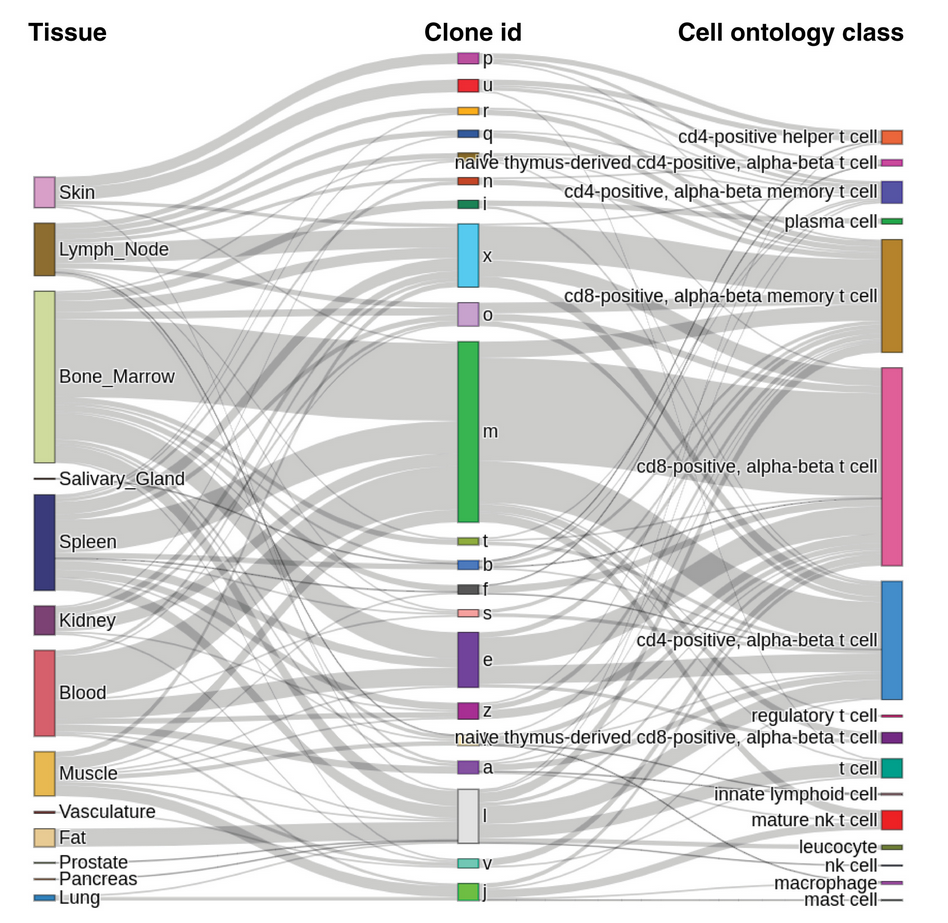
\includegraphics[width=14cm, keepaspectratio]{figs/paper1/fig4_sankey.png}
\caption[Sankey Plot of T cell clones in Tabula Sapiens]{Illustration of clonal distribution of T cells across multiple tissues. The majority of T cell clones are found in multiple tissues and represent a variety of T cell subtypes. nk cell, natural killer cell.}
\label{fig:paper1_sankey}
\end{figure}


\subsection{Cross-Referencing TCR/Epitope Pairings with Tabula Sapiens Database}

We downloaded a curated database of TCR/epitope pairings containing 54,181 unique CDR3-to-epitope pairings. The majority of these pairings are supported by evidence from dextramer, tetramer, or multimer sorting and subsequent sequencing. In some cases, this data is derived from single-cell analysis, while in others, it is based on bulk RNA. We then cross-referenced this database with the Tabula Sapiens database of TCRs that we generated. Upon cross-referencing, we identified 25 TCR Beta Chains with exact matches in the database describing TCR/epitope pairings. This represents roughly 1/100 of the TCRBs in Tabula Sapiens. We were able to identify T cells which likely bind to viruses, specifically:
\begin{itemize}
\item Epstein-Barr Virus (EBV): 12 peptides
\item Cytomegalovirus (CMV): 8 peptides
\item Influenza A: 5 peptides
\end{itemize}

\subsection{Distribution of Virus-Binding T Cells}
The EBV-binding T cells were found in donors TSP2 and TSP7. In TSP7, the single EBV-specific T cell was located in the tongue. In TSP2, EBV-specific T cells were distributed amongst multiple immune organs. We could not perform any meaningful statistical comparison with such low numbers of cells.(Fig 2.4).
\subsection{Isotype Distribution in B Cells Across Tissues}

B cells secrete different isotypes of the IgH gene, which have different roles in immunity. IgA interacts with pathogens and commensals at mucosal surfaces, IgG is often involved in direct neutralization of pathogens, and IgM is typically expressed in naive B cells or secreted in the first response to pathogens. We classified every B cell in the dataset as expressing IgA, IgG, or IgM and calculated the relative amounts of each isotype in each tissue. This analysis revealed a gradient of IgA expression across tissues, with blood having the least relative abundance of IgA cells and the large intestine having the highest relative abundance \ref{fig:paper1_igh}.

\subsection{Tissue-Specific Somatic Hypermutation in B Cells}

We measured the level of tissue-specific somatic hypermutation in B cells by computationally assembling the B Cell Receptor (BCR) and then inferring the germline ancestor of each cell\cite{lindeman2018bracer,gupta2015change}. In the bone marrow, we observed a bimodal distribution of hypermutation, consistent with the coexistence of plasma cells and recently birthed B cells \ref{fig:paper1_igh}. Solid tissues have an order of magnitude higher level of mutations per nucleotide (0.07 ±0.04) compared to the blood (0.007±0.02), suggesting that immune infiltrates of solid tissues are dominated by antigen experienced B cells.

\begin{figure}[hbt!]
\centering
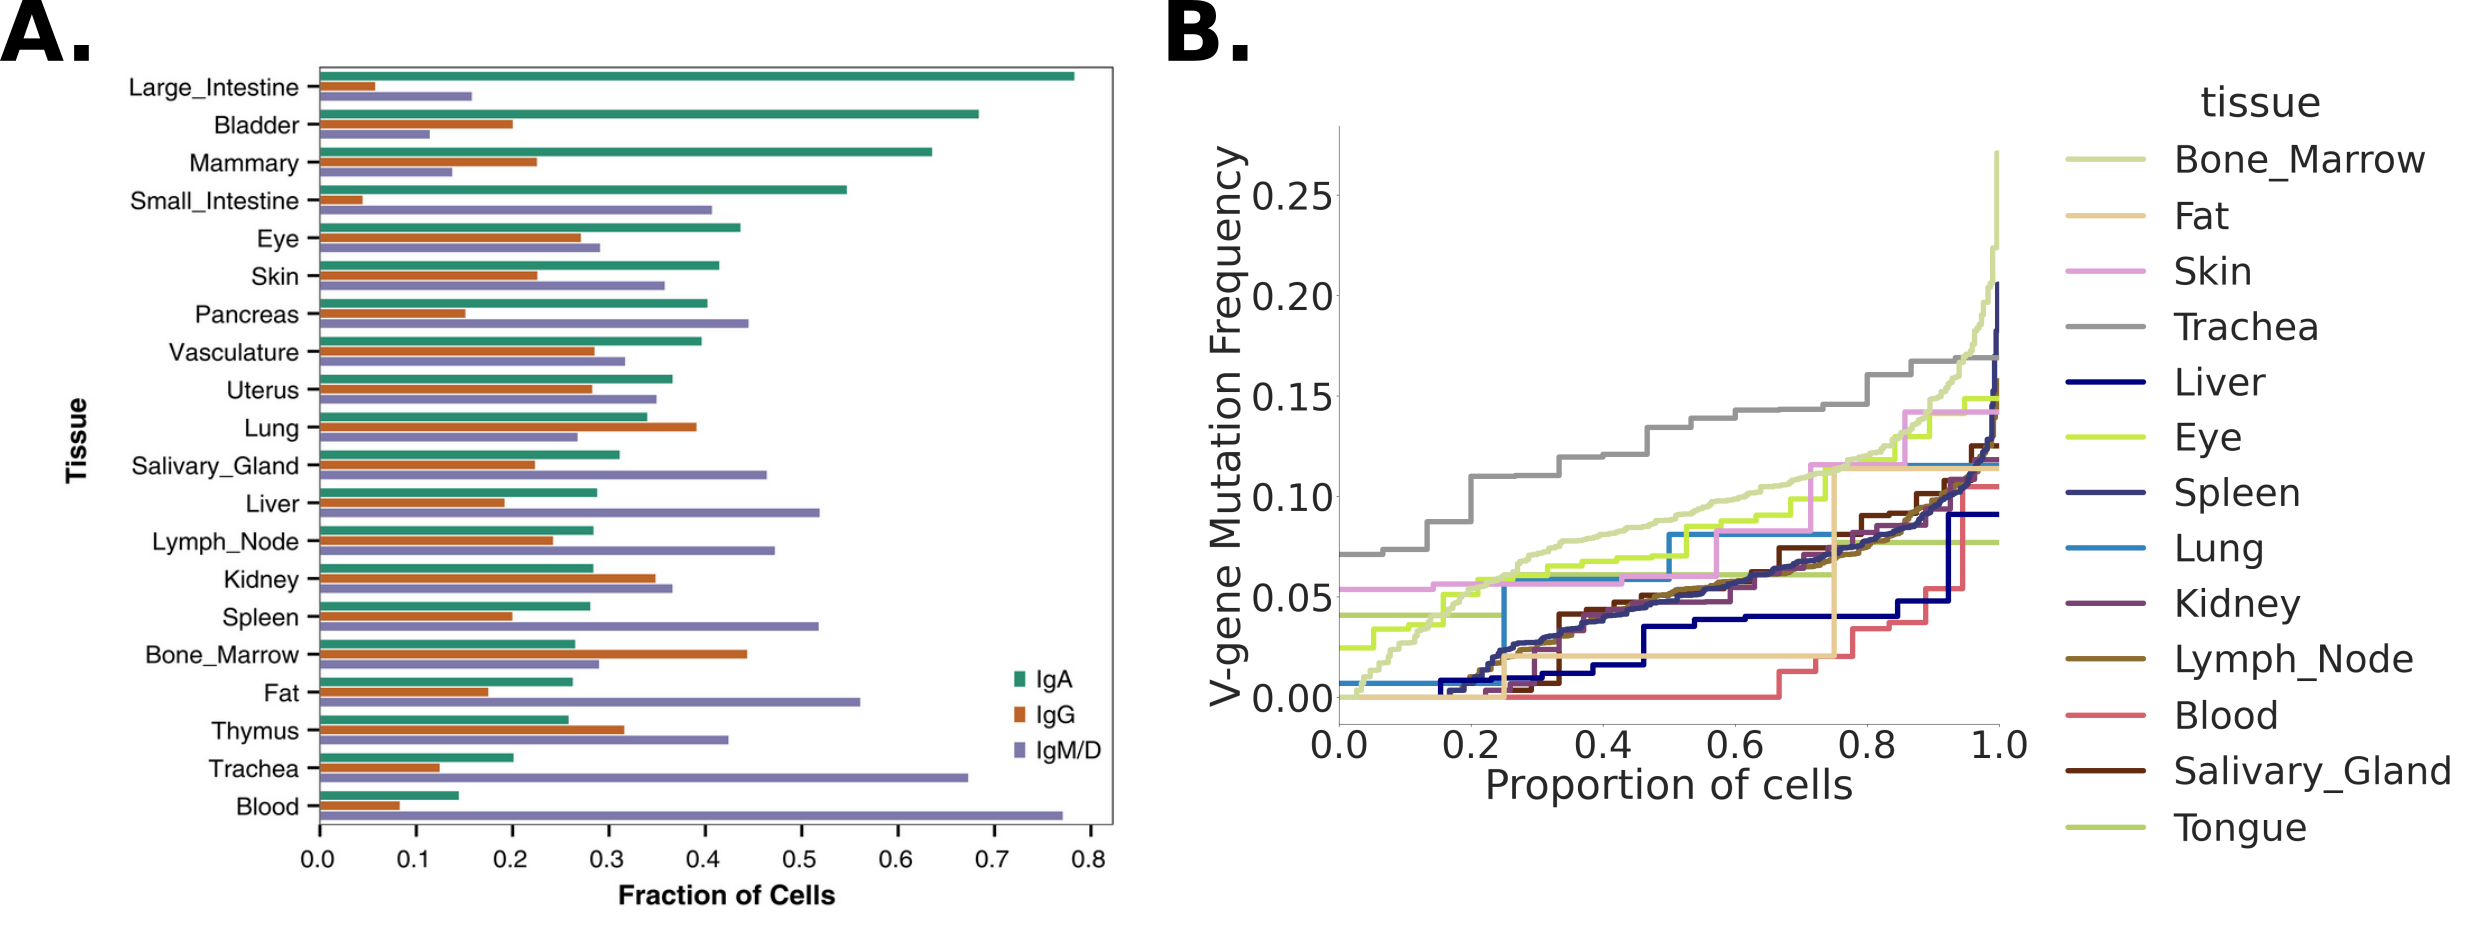
\includegraphics[width=14cm, keepaspectratio]{figs/paper1/fig3_tabula_igh.png}
\caption[Tissue population-level parameters of B cell Dynamics.]{(A) Prevalence of B cell isotypes across tissues, ordered by decreasing abundance of IgA (B) Somatic hypermutation frequencies in the V-genes of B cells sampled from different tissues in
Tabula Sapiens.}
\label{fig:paper1_igh}
\end{figure}

\section{Conclusions}

Our results provide valuable insights into immune cell trafficking, tissue-specific gene expression signatures, and the distribution of virus-binding T cells across different tissues. Furthermore, our findings shed light on the tissue-specific somatic hypermutation in B cells and the distribution of B cell isotypes across various tissues.
We observed tissue-specific gene expression signatures in immune cells, notably macrophages, and identified gradients of EREG expression that distinguished tissue-resident macrophages from circulating ones. We also found tissue-specific differences in B cell somatic hypermutation and isotype distribution.
These findings have important implications for understanding immune cell trafficking and the molecular mechanisms governing immune cell differentiation and function. Further investigation is necessary to validate and expand upon these results, as well as to explore potential clinical applications and therapies that may arise from this knowledge.

\section{Materials and Methods}
\subsection{Vertebral Body Tissue Processing}
The vertebral bodies (VB) were wrapped in a cloth and shipped to Stanford University on ice.
Upon arrival, the VBs were first cleaned using chisels, to remove any attached connective tissue
and fat. To rinse off any remaining cells attached to the exterior of the VB, the VBs were then
transferred to a plastic nalgene containing 50 mL RPMI + 10\% FBS and tumbled in a bone marrow
tumbler for 20 minutes at room temperature. The rinsing medium was discarded and the VBs
were removed from the tumbler, transferred to a large sterile plastic Petri dish, and cut into ½ inch
by ½ inch pieces using bone cutting forceps. The bone marrow pieces were transferred into a
plastic nalgene, to which 100mL of RPMI + 10\% FBS was added. The nalgene was returned to
the bone marrow tumbler and tumbled for 30 minutes at room temperature. The solution
containing the VB was then passed through a 100 $\mu$M strainer into 50 mL falcon tubes. Multiple
strainers were used in case of clogs. After straining, the cells were centrifuged and pelleted at
330g 4°C for 5 minutes. Cells were resuspended in 1x Erythrocyte Lysis buffer, kept 5 minutes
on ice and mixed. Cells were then re-centrifuged for 5 minutes at 330g at 4°C without brakes, in
order to remove plasma and lysed red blood cells. Cells were then ready to count. 10 million bone
marrow cells were stained using an immune lineagePE cocktail containing CD3-PE, CD4-PE,
CD56-PE, CD11b-PE, and CD14-PE, and subsequent MACS with anti-PE microbeads was
performed. One tube of immune lineage positive and one tube of lineage negative cell were
prepared for the 10x. For smartseq2, cells were stained with anti-CD38-APC, anti-CD34-FITC,
and sytox blue for 30 minutes at 4°C and washed twice with PBS + 10\% FBS. A more detailed protocol may be found on protocols.io. 